\fontsize{9}{10.5}\selectfont
\par\Needspace{100pt}\section*{Older Q1: Use-case models and descriptions}\label{older-q1}
\phantomsection\addcontentsline{toc}{section}{Older Q1: Use-case models and descriptions}
\markboth{Older papers | Q1}{}
\textbf{Shared method:} use the boundary/relationship and description checks in Chapter 3, p.\ \pageref{chapter-3}. Each case retains its own actors, flow and failure rules.
\par\Needspace{85pt}\subsection*{AY2022/23 S1: Car sales --- Q1 (25 marks)}\label{old-2223-s1-q1}

\sectionlabel{h-q1--use-cases-25-marks}
\textbf{(a) Identify actors/\allowbreak{}use cases and draw their relationships (17). (b) Describe holding a car: actors, preconditions, flow and alternatives (8).}


\textbf{(a)} Actors: Visitor, Registered Customer, Dealer Staff, Sales Manager and external Dealer Payment System. Registered Customer can do the visitor's browsing; Sales Manager inherits staff capabilities. The system itself, its database and a car are not actors.





\par\smallskip\noindent\begin{minipage}{\linewidth}\centering
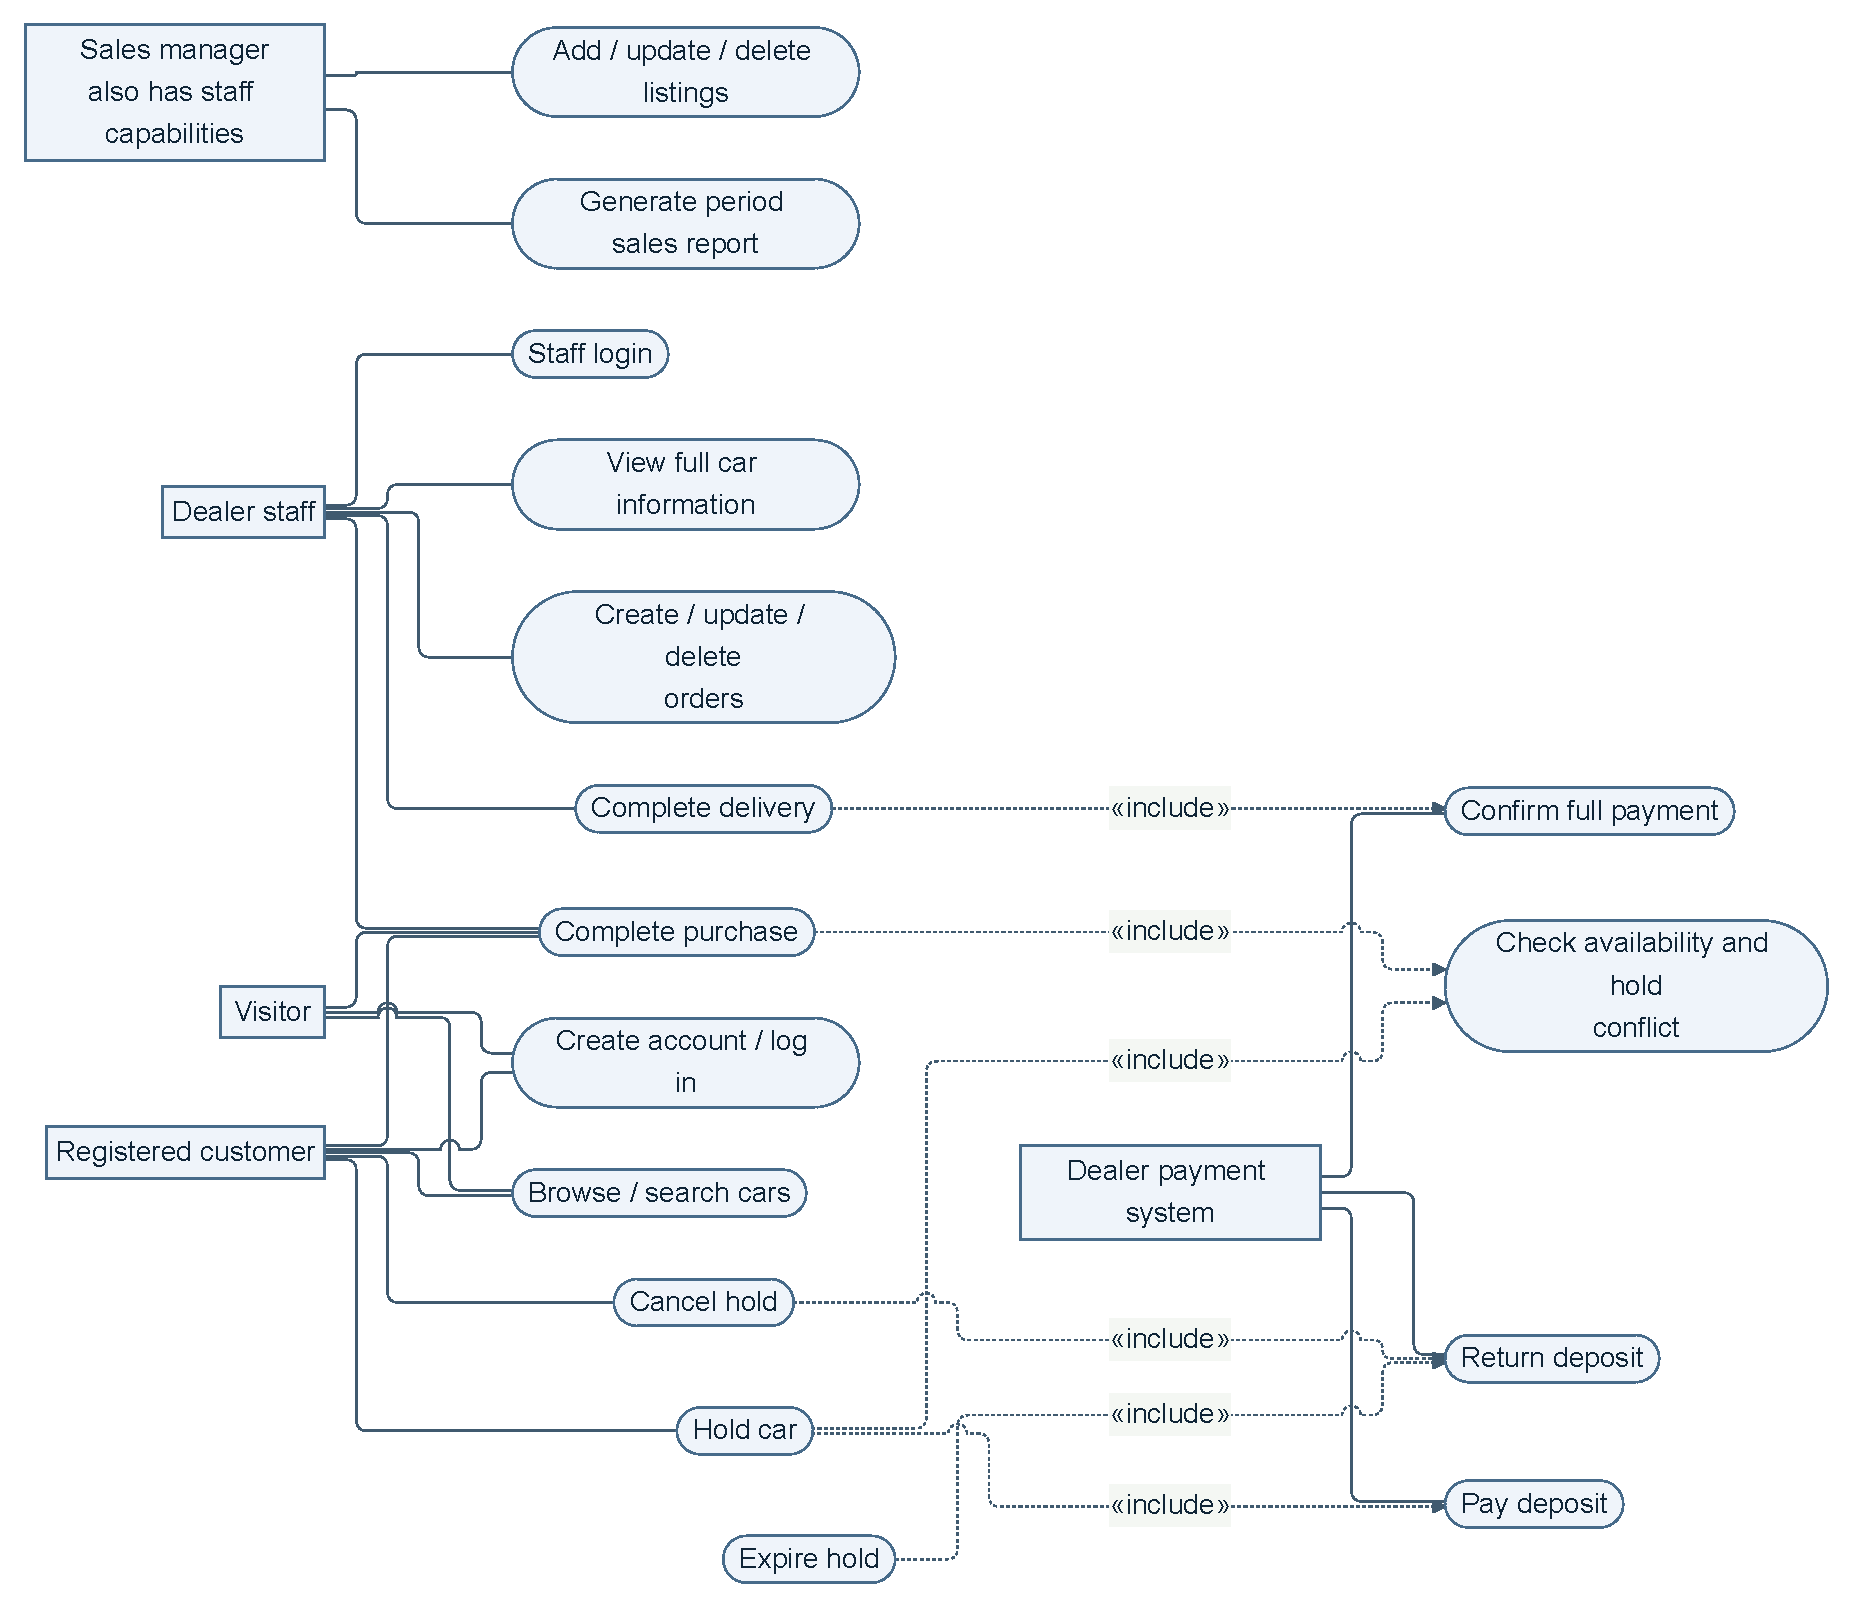
\includegraphics[width=506.64pt]{images/fig-048.pdf}
\captionof{figure}{Car sales: Q1 --- Use cases (25 marks)}\end{minipage}\par\smallskip

\begin{studycolumns}
\vspace{0pt}




Generalization: Customer to Visitor; Sales Manager to Staff. Expiry is an internally scheduled system action; a timer need not be invented as an external actor. The appendix does not explicitly require an account/\allowbreak{}deposit for a direct purchase with staff; those requirements apply to holding a car. A failed deposit is an alternative flow. The question says use relationships \textbf{where appropriate}, so an artificial extension is unnecessary.

\textbf{(b) Use case: Hold Car.} Primary actor: Registered Customer. Supporting actor: Dealer Payment System. Preconditions: customer is authenticated; selected car exists, is unsold and is not already under an active hold. Normal flow:

\begin{enumerate}
\item Customer selects a car and requests a hold.
\item System checks current availability and displays deposit/\allowbreak{}hold terms. The duration and deposit amount come from dealer policy; the paper gives no numbers.
\item Customer confirms and authorises the deposit through the payment system.
\item Payment system confirms success. System creates the hold for that customer and marks the car unavailable to other customers until expiry.
\item System displays the hold reference and expiry time.
\end{enumerate}
Alternatives: failed/\allowbreak{}cancelled payment creates no active hold; a concurrent hold/\allowbreak{}purchase causes rejection rather than double allocation; expiry or user cancellation ends the hold and requests a refund. A payment confirmed after an allocation conflict must be compensated/\allowbreak{}refunded. \textbf{Design assumption:} availability checks and allocation are made atomic, with a pending reservation/\allowbreak{}payment reconciliation mechanism. Do not imply that an initial availability check alone prevents races.
\end{studycolumns}

\par\Needspace{85pt}\subsection*{AY2022/23 S2: Shopping chatbot --- Q1 (25 marks)}\label{old-2223-s2-q1}


\begin{studycolumns}
\vspace{0pt}
\sectionlabel{h-q1--use-cases-25-marks-1}
\textbf{(a) Actors/\allowbreak{}use cases and relationships (17). (b) Item-replacement description with actors, preconditions, normal/\allowbreak{}alternative flows (8).}


\textbf{(a)} The chatbot is the system being modelled, not an external actor. Customer is the primary actor. Existing Web-Based Shopping System is a supporting actor outside the chatbot boundary; company approval is supplied through that system. If company staff directly operate a chatbot approval interface, they become another actor, but that interface is not specified.
\end{studycolumns}


\par\smallskip\noindent\begin{minipage}{\linewidth}\centering
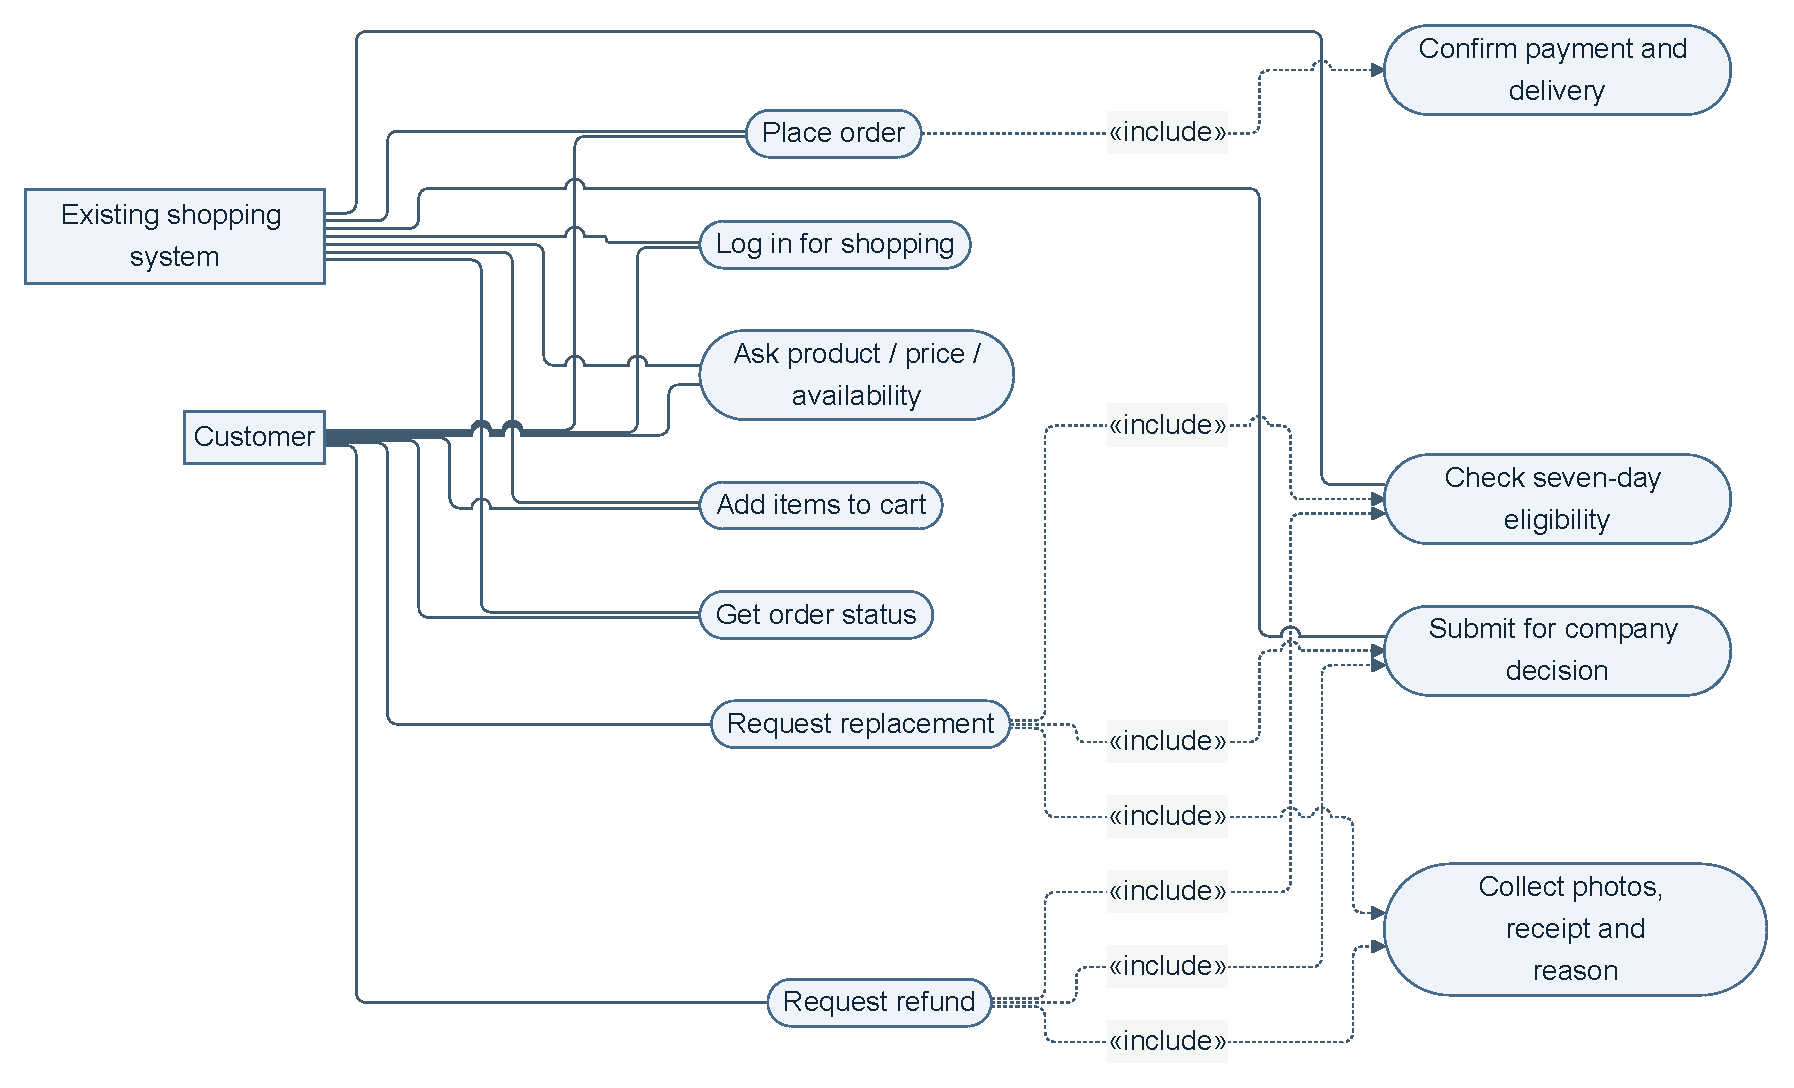
\includegraphics[width=461.44pt]{images/fig-053.pdf}
\captionof{figure}{Shopping chatbot: Q1 --- Use cases (25 marks)}\end{minipage}\par\smallskip

\begin{studycolumns}
\vspace{0pt}



Approval leads to replacement/refund instructions; rejection is an alternative flow. Shopping actions require a valid authenticated session, while product enquiries can precede login.

\textbf{(b) Use case: Request Item Replacement.} Actors: Customer, Existing Shopping System (including company decision service). Preconditions: customer is logged in; the delivered purchase can be identified. Normal flow:

\begin{enumerate}
\item Customer asks for replacement and selects the purchased item/\allowbreak{}order.
\item Chatbot retrieves purchase/\allowbreak{}delivery details and checks the seven-day rule.
\item Chatbot asks for item photos, receipt and replacement reason; customer supplies them.
\item Chatbot validates completeness and submits the request to the existing system for company confirmation.
\item On approval, chatbot sends the company-provided replacement procedure and request reference.
\end{enumerate}
Alternatives: outside the eligibility period, reject the free replacement; missing evidence, request correction; company rejects, communicate rejection; integration failure, report pending/\allowbreak{}failure without falsely confirming approval. \textbf{Assumption:} ``within seven days'' includes the seventh day; the exact timestamp/\allowbreak{}timezone policy needs agreement. Company review may be asynchronous, so ``submitted/\allowbreak{}pending'' is distinct from ``approved''.
\end{studycolumns}

\par\Needspace{85pt}\subsection*{AY2023/24 S1: DevSecOps --- Q1 (25 marks)}\label{old-2324-s1-q1}

\sectionlabel{h-q1--use-cases-25-marks-2}
\textbf{(a) Actors, use cases and relationships (17). (b) Describe the security-check functionality (8).}


\textbf{(a)} Primary actor: Developer. Supporting actors: external SCA/\allowbreak{}SAST/\allowbreak{}DAST/\allowbreak{}IAST services and GitHub for remote project retrieval. The platform's own scanner coordinator and report store are internal components, not actors.




\par\smallskip\noindent\begin{minipage}{\linewidth}\centering
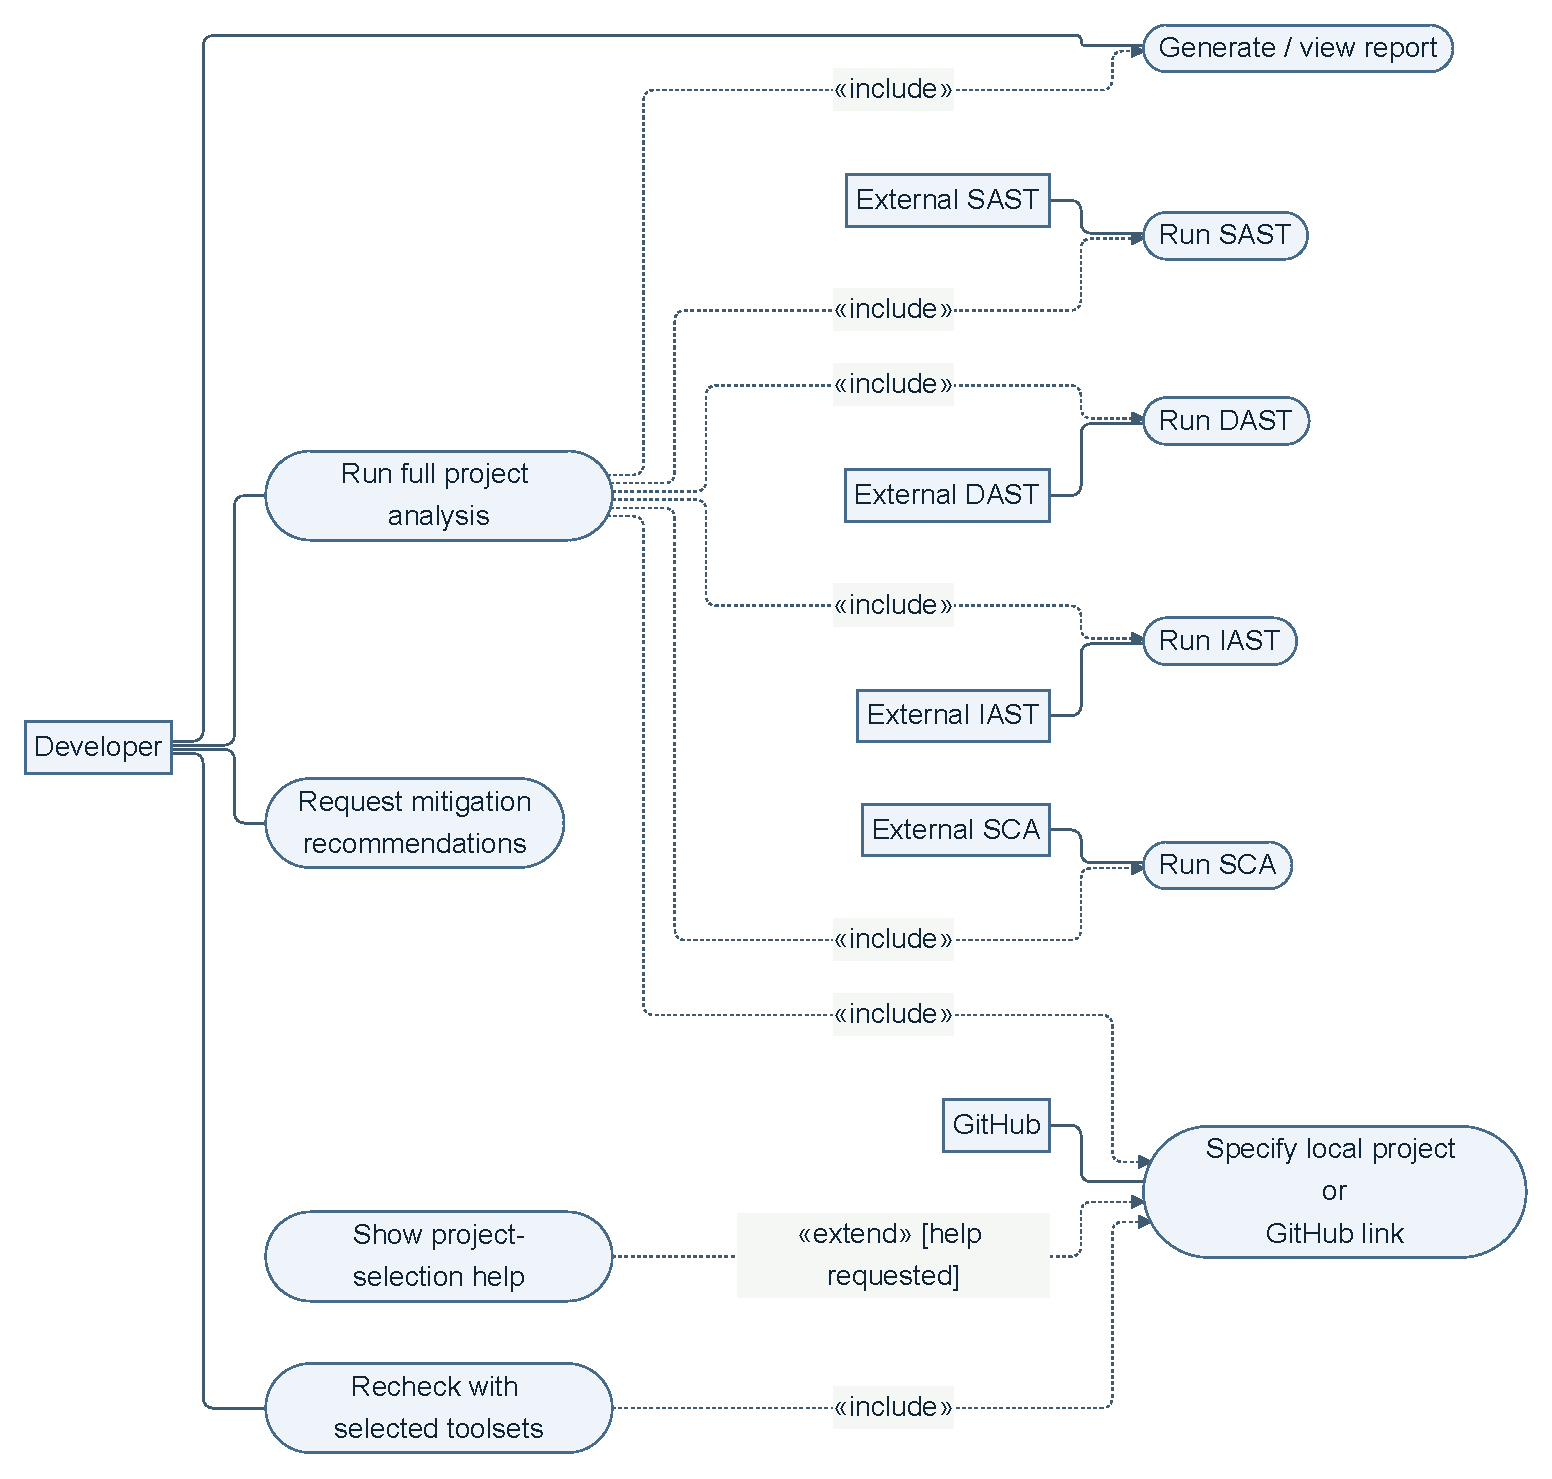
\includegraphics[width=436.92pt]{images/fig-058.pdf}
\captionof{figure}{DevSecOps: Q1 --- Use cases (25 marks)}\end{minipage}\par\smallskip

\begin{studycolumns}
\vspace{0pt}



Selected reruns invoke only chosen engines; the diagram's four mandatory includes apply to the \textbf{full-analysis} use case. GitHub participates only in the remote-source alternative. Mitigation is available after a report; it need not be automatically included in every scan. Selection help is a genuine optional extension.

\textbf{(b) Use case: Check Project Security.} Actors: Developer; selected external analysis toolsets; GitHub when applicable. Preconditions: project is accessible; required engines are available/\allowbreak{}configured. Normal flow:

\begin{enumerate}
\item Developer specifies local source or a GitHub link; platform obtains the project.
\item Platform runs all four toolsets for an initial full analysis, or the developer selects toolsets for a verification rerun.
\item Each selected toolset returns its findings; platform associates results with the project/\allowbreak{}version and combines them.
\item Platform generates and displays a security/\allowbreak{}quality report.
\item On request, platform supplies mitigation recommendations.
\end{enumerate}
Alternatives: developer requests selection help; inaccessible source produces a corrective message; unsupported/\allowbreak{}failed/\allowbreak{}timed-out engine is reported with explicit incomplete status, not a clean result; developer fixes issues and reruns selected checks. Version tagging and incomplete-result status are proposed design details needed for trustworthy results. The paper does not specify a login requirement, so do not invent one as a case fact.
\end{studycolumns}

\par\Needspace{85pt}\subsection*{AY2023/24 S2: CodeAgent --- Q1 (25 marks)}\label{old-2324-s2-q1}

\sectionlabel{h-q1--use-cases-25-marks-3}
\textbf{(a) Actors/\allowbreak{}use cases/\allowbreak{}relationships (19). (b) Reviewer-agent use case description (6).}


\textbf{(a)} With the \textbf{whole CodeAgent platform} as the system boundary, agents are internal software, not external human actors. Model the six corresponding external user roles and their authenticated interactions. Appendix wording is unusual; this boundary/\allowbreak{}role interpretation is explicit rather than silently treating every program as an actor.







\par\smallskip\noindent\begin{minipage}{\linewidth}\centering
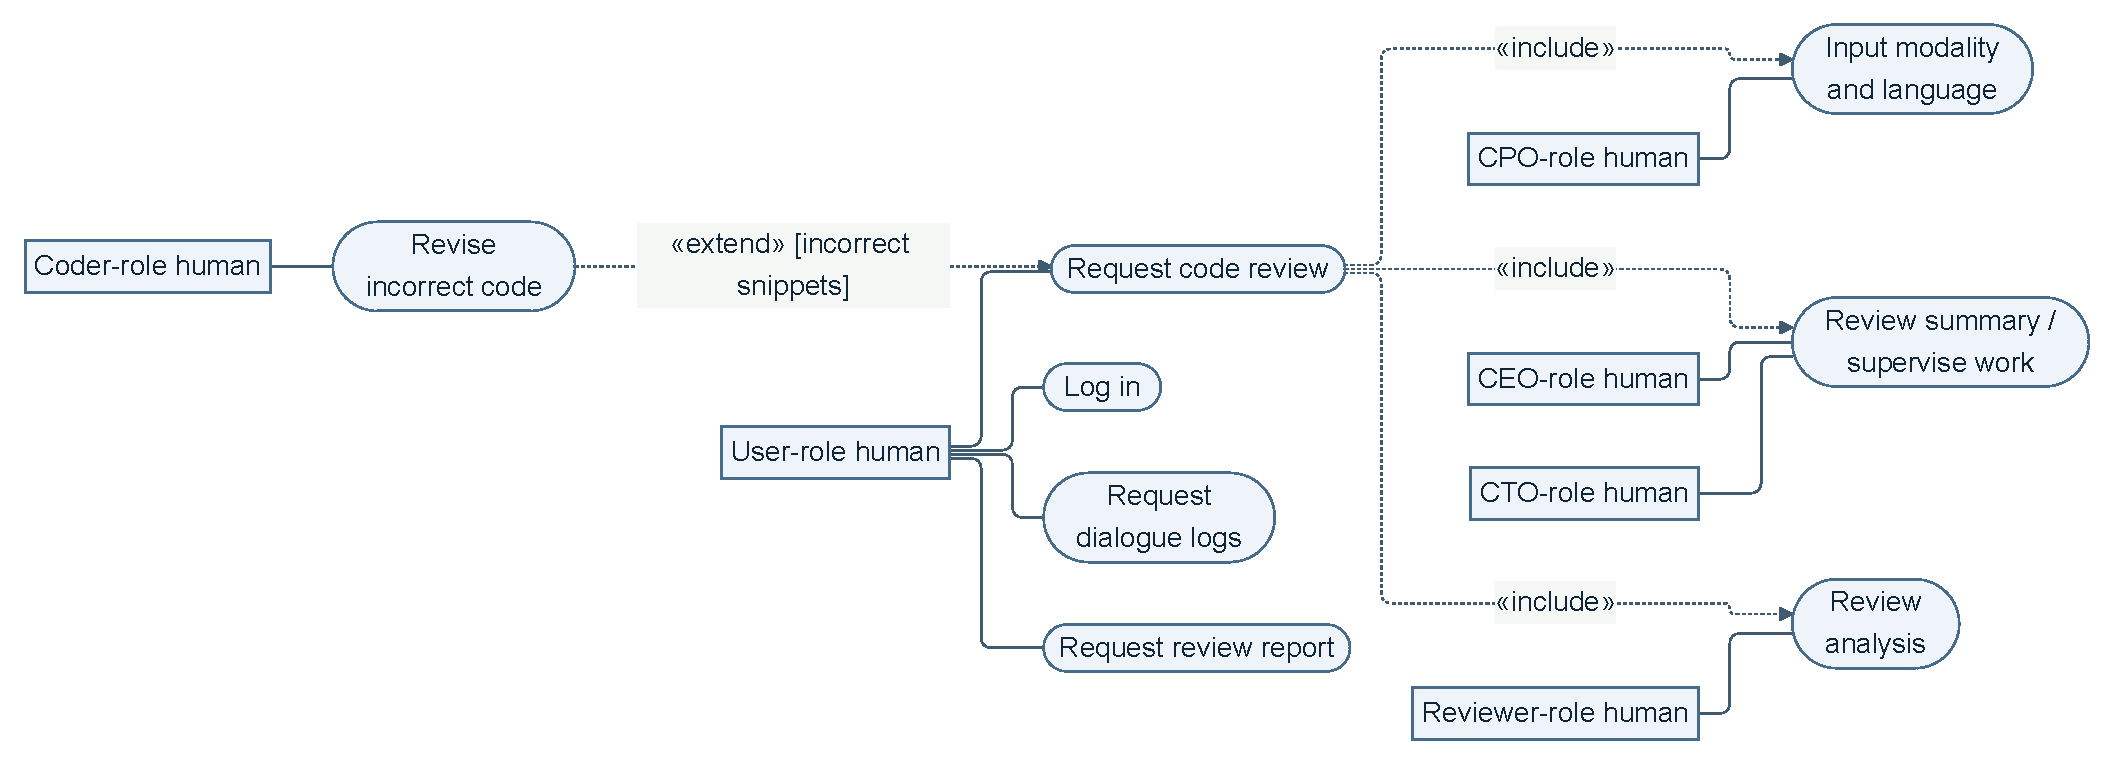
\includegraphics[width=514.00pt]{images/fig-063.pdf}
\captionof{figure}{CodeAgent: Q1 --- Use cases (25 marks)}\end{minipage}\par\smallskip





Detail view of the same \textbf{Perform review analysis} use case:




\par\smallskip\noindent\begin{minipage}{\linewidth}\centering
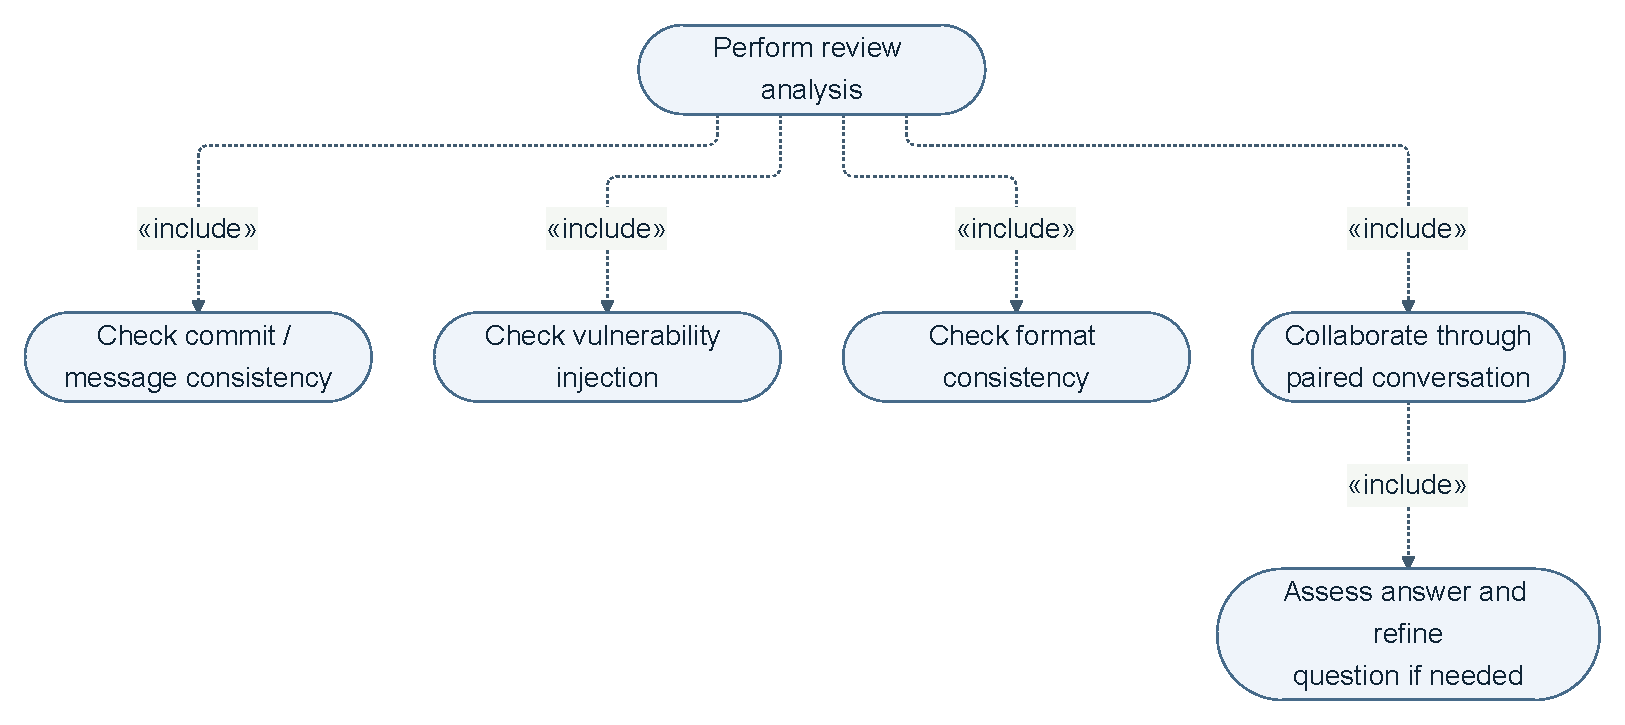
\includegraphics[width=457.60pt]{images/fig-064.pdf}
\captionof{figure}{CodeAgent: Q1 --- Use cases (25 marks)}\end{minipage}\par\smallskip

\begin{studycolumns}
\vspace{0pt}



All six role users can log in, interact with their corresponding agents, and request permitted outputs; show generalization to a common Authenticated User actor in exact UML rather than implying that only User-role humans log in. Internal CEO/\allowbreak{}CPO/\allowbreak{}Coder collaboration and Coder/\allowbreak{}CTO/\allowbreak{}CEO summarisation occur through agent orchestration; external users need not manually perform every subtask. QA-Checker needs no extra human actor.

\textbf{(b) Use case: Review Submitted Code.} Primary actor: authenticated requesting user/\allowbreak{}Reviewer-role user, according to the interface boundary chosen above. Preconditions: commit, commit message and original files are available; prior input recognition identifies modality/\allowbreak{}language. Flow: submit review request; Reviewer obtains code/\allowbreak{}context with Coder's help; analyse commit-message consistency, introduced vulnerabilities and formatting; conduct supervised conversations where needed; create an analysis report with observations and suggested revisions; provide it to Coder/\allowbreak{}user. Alternatives: missing/\allowbreak{}unreadable inputs, ask for correction; inappropriate answers, QA-Checker appends instructions and retries within the limit; limit exhausted, report unresolved/\allowbreak{}incomplete analysis rather than claiming success. Coder's subsequent revision is conditional on finding incorrect snippets.
\end{studycolumns}

